\documentclass[11pt]{article}

%%%%%%%%%%%%
% Packages %
%%%%%%%%%%%%
\hyphenpenalty=10000
\usepackage{tocloft}
\renewcommand\cftsecleader{\cftdotfill{\cftdotsep}}

\usepackage{xcolor}
\usepackage{hyperref}
\usepackage{epstopdf}
\usepackage{braket}
\usepackage{upgreek}
\usepackage{caption}
\usepackage{booktabs}
\usepackage{subcaption}
\usepackage{amssymb,latexsym,amsmath,gensymb}
\usepackage{latexsym}
\usepackage{graphicx}
\usepackage{float}
\usepackage{enumitem}
\usepackage{pdflscape}
\usepackage{url}
\usepackage{tikz, calc}
\usetikzlibrary{shapes.geometric, arrows, calc}
\tikzstyle{norm} = [rectangle, rounded corners, minimum width=2cm, minimum height=1cm,text centered, draw=black]
\tikzstyle{arrow} = [thick, ->, >=stealth]

\providecommand{\e}[1]{\ensuremath{\times 10^{#1}}} 
\providecommand{\mb}[1]{\mathbf{#1}}
\providecommand{\mh}[1]{\mathbf{\hat{#1}}}
\providecommand{\bs}[1]{\boldsymbol{#1}} 
\providecommand{\intinf}{\int_{-\infty}^{\infty}}
\providecommand{\fig}[4]{
  % filename, width, caption, label
\begin{figure}[h]
 \captionsetup{width=1.0\linewidth}
 \centering
 \includegraphics[width = #2\textwidth]{#1}
 \caption{#3}
 \label{fig:#4}
\end{figure}
}

\newcommand{\tensor}[1]{\overset{\text{\tiny$\leftrightarrow$}}{\mb{#1}}}
\newcommand{\tunderbrace}[2]{\underbrace{#1}_{\textstyle#2}}
\providecommand{\figs}[7]{
  % filename1, filename2, caption1, caption2, label1, label2, shift
\begin{figure}[H]
\centering
\begin{minipage}[b]{.4\textwidth}
  \centering
  \includegraphics[width=1.0\linewidth]{#1}
  \captionsetup{justification=justified, singlelinecheck=true}
  \caption{#3}
  \label{fig:#5}
\end{minipage}
\hspace{2em}
\begin{minipage}[b]{.4\textwidth}
  \centering
  \includegraphics[width=1.0\linewidth]{#2}
  \vspace{#7em}
  \captionsetup{justification=justified}
  \caption{#4}
  \label{fig:#6}
\end{minipage}
\end{figure}
}
\makeatletter

\providecommand{\code}[1]{
\begin{center}
\lstinputlisting{#1}
\end{center}
}

%%%%%%%%%%%
% Spacing %
%%%%%%%%%%%
% Margins
\usepackage[
top    = 1.5cm,
bottom = 1.5cm,
left   = 1.5cm,
right  = 1.5cm]{geometry}

% Indents, paragraph space
\usepackage{parskip} 

% Section spacing
\usepackage{titlesec}
\titlespacing*{\title}
{0pt}{0ex}{0ex}
\titlespacing*{\section}
{0pt}{0ex}{0ex}
\titlespacing*{\subsection}
{0pt}{0ex}{0ex}
\titlespacing*{\subsubsection}
{0pt}{0ex}{0ex}

% Line spacing
\linespread{1.1}

%%%%%%%%%%%%
% Document %
%%%%%%%%%%%%
\begin{document}
\title{\vspace{-2.5em}Single Molecule Fluorescence Microscopy Notes\vspace{-1em}}
\author{Talon Chandler}% and Patrick La Rivi\`ere}
\date{\vspace{-1em}February 10, 2017\vspace{-1em}}
\maketitle

\section{Introduction}
These notes develop the forward model for a wide class of single molecule
fluorescence microscopes. We split the imaging process into four
parts---illumination, excitation, emission, and detection---and analyze each
part individually. For each part of the imaging process, we will perform a
general analysis, relate the analysis to current techniques, and mention
possible improvements.

\subsection{Notation}
We use boldface for vectors $\mathbf{r}$, hats for unit vectors
$\mathbf{\hat{r}}$, normal face for vector lengths $r = |\mathbf{r}|$, tildes
for matrices $\mb{\tilde{O}}$, and double arrows for tensors $\tensor{\mb{G}}$.

\subsection{Coordinates}
First, we place the origin at the geometric focus of the microscope. If there
are multiple objectives we assume that the foci are perfectly aligned. Next, we
choose a fixed laboratory coordinate system using Cartesian unit vectors
$\mb{r} = x\mh{x} + y\mh{y} + z\mh{z}$.


\section{Illumination}
\subsection{General Analysis}
We view illumination as the process of establishing an electric field
distribution $\mb{E}(\mb{r}, t)$ near the origin. In these notes we
will use the complex spatial electric field $\mb{E}(\mb{r})$ related to the
time dependent electric field by
\begin{align*}
  \mb{E}(\mb{r}, t) = \text{Re}\{\mb{E}(\mb{r})e^{-j\omega t}\}. 
\end{align*}
We will refer to the complex spatial electric field as the electric field.
Analysis of the illumination pattern consists of finding the input electric field
$\mb{E}_{\text{in}}(\mb{r})$ near the focal point.

\subsection{Current Techniques}
\subsubsection{Laser K\"{o}hler Illumination}
Laser K\"{o}hler illumination is accomplished by focusing a laser beam onto the
center of the back focal plane of the objective as shown in Figure 2(a) of
\cite{backlund}. Under laser K\"{o}hler illumination a constant electric field
is established in the focal region. That is
\begin{align*}
  \mb{E}_{\text{in}}(\mb{r}) = \mb{P}
\end{align*}
where $\mb{P}$ is the 3D vector pointing along the polarization direction of the
laser. Under laser K\"{o}hler illumination the electric field in the focal
region is always transverse, and the electric field is constant throughout the
field of view.

If we use a modulated polarizing element on the illumination side, its pass
direction will change $\mb{P}$.

Notice that both $\mb{E}$ and $\mb{P}$ are 3D vectors, not 2D Jones vectors. We
will continue using 3D vectors throughout these notes so that we can consider
illumination patterns from any angle.

\subsubsection{Laser Critical Illumination}
Laser critical illumination is accomplished by illuminating the entire back
focal plane of the objective with a laser as shown in shown in Figure 2b) of
\cite{backlund}. Under laser critical illumination, the electric field varies
near the focal plane. The electric field at every point can be calculated using
the Richards-Wolf diffraction integral \cite{richards}. To calculate the
electric field at a point we calculate the electric field at that point due to a
single point on the lens, then integrate the contributions from each point while
keeping track of the phase to allow for interference. See Chapter 3 of
\cite{nov} for a complete calculation of the focal fields created by a spherical
lens including consideration of under filling the back aperture and higher order
laser modes.

If the back aperture receives uniform illumination, then the electric fields in
the focal plane will be transverse and the electric fields away from the focal
plane will have a transverse component. See Figures 8-10 of \cite{youngworth} for
images of the fields.

Laser critical illumination only creates an appreciable electric field near the
focal spot, so an image must be built up by scanning. 

We can also illuminate the sample with a cylindrical lens. The electric field
pattern created by a cylindrical lens can be found in \cite{youngworth}.

Under laser critical illumination the electric field near the focal plane can be
modified by modulating the intensity and phase in the back focal plane.
Axial patterning, radial patterning, and ``bone'' patterning are some modulation
patterns that have been explored \cite{debarre}.

\subsection{Possible Techniques}
\subsubsection{Lamp Illumination}
Lamp illumination could be used to provide inexpensive and novel illumination
patterns. Under laser illumination we can establish a fixed electric field
distribution, but under lamp illumination we need to consider the electric field
at each point as a vector stochastic process. Analyzing the vector stochastic
process requires a statistical optics approach that includes polarization
effects.

The complete theory of coherence and polarization was completed in 2003
\cite{wolf}, and has not, to my knowledge, been applied to single molecule
microscopy problems.

\section{Excitation}
\subsection{General Analysis}
Consider a two-level quantum system in the dipole approximation---an excellent
model for many fluorophores. Each transition can be described by a
\textit{transition dipole moment}, a vector that points in a fixed direction
with respect to the molecule's molecular structure. We denote the absorption
dipole moment by $\bs{\mu}_{\text{abs}}$ (called $\bs{\mu}_{21}$ in quantum
mechanics) and the emission dipole moment by $\bs{\mu}_{\text{em}}$
($\bs{\mu}_{12}$). The transition dipole moments can be calculated analytically
for simple systems using quantum mechanics, calculated numerically for complex
systems using Hartree-Fock theory or density functional theory, or measured
experimentally. 

When a fluorophore with transition dipole moments $\bs{\mu}_{\text{em}}$ and
$\bs{\mu}_{\text{abs}}$ is exposed to a weak electric field $\mb{E}$ that is
constant near the fluorophore, the electric field creates an
$\textit{induced dipole moment}$$\ \bs{\mu}$ where
\begin{align*}
  \bs{\mu} \propto \bs{\mu}_{\text{em}}\bs{\mu}_{\text{abs}}^{\dagger}\mb{E}_{\text{in}}. 
\end{align*}
The relationship between the incident electric field and the induced dipole
moment is summarized by the \textit{polarizability tensor}
$\tensor{\bs{\alpha}}$ where
\begin{align*}
  \bs{\mu} &= \tensor{\bs{\alpha}}\mb{E}_{\text{in}}\\
  \tensor{\bs{\alpha}} &\propto \bs{\mu}_{\text{em}}\bs{\mu}_{\text{abs}}^{\dagger}
\end{align*}

If we assume $\bs{\mu}_{\text{em}}
=\bs{\mu}_{\text{abs}}$ then the induced dipole can only be created along a
single axis relative to the molecule's structure. This assumption is invalid for
many fluorophores---even GFP's transition dipole moments are a few degrees apart
\cite{rosell2003}. Some crystals have excitation and emission transition dipole
moments that are orthogonal \cite{koberling}!

General reference for this section: Appendix A of \cite{nov}.

\subsection{Current Techniques}
Many single molecule orientation and location estimation experiments make the
unstated assumption that $\bs{\mu}_{\text{em}} =\bs{\mu}_{\text{abs}}$. Under
this assumption, the induced dipole direction is identical to the directions of
the transition dipole moments. 


Many groups approach the excitation analysis from a ``power absorbed'' or a
``probability'' viewpoint. In the their 2014 review \cite{backer}, the Moerner
group says that ``the probability of absorption is proportional to
$|\bs{\mu}_{\text{abs}}\cdot\mb{E}|^2$''. This approach is identical to the
induced dipole approach above. We deal with classical electric fields and
induced dipole moments, while they deal with probabilities of photon absorption. We
will take the modulus squared of the electric field during detection, so the
approaches are identical. 

\subsection{Possible Techniques}
\subsubsection{Estimating The Induced Dipole Moment}
With the analysis above, we can attempt to estimate the complete induced dipole
moment, not just the orientation of the induced dipole moment. 

\subsubsection{Simultaneous Analysis of Illumination and Detection}
Estimating the induced dipole moment allows us to simultaneously analyze the
illumination and detection paths. To my knowledge, the illumination and
detection paths have only been considered individually. A simultaneous analysis
could allow us to find unique ways of modulating the illumination and detection
paths together.

\subsubsection{Estimating Both Transition Dipole Moments}
If $\bs{\mu}_{\text{em}} \neq\bs{\mu}_{\text{abs}}$, then we may find techniques
for simultaneously measuring both $\bs{\mu}_{\text{em}}$ and
$\bs{\mu}_{\text{abs}}$. Measured both transition dipole moments could be useful
for characterizing fluorophore and for measuring the effects of an environment on
a fluorophore. 

\section{Emission}
\subsection{General Analysis}
\fig{../figures/locations/locations.pdf}{.27}{Position and orientation
  vectors.}{locations} Consider an induced dipole moment $\bs{\mu}$ at
$\mathbf{r}'$ in a medium with index of refraction $n_1$ with an as shown in
Figure \ref{fig:locations}. The electric field distribution $\mathbf{E}_{\text{obj}}(\mb{r})$ is related to $\mathbf{r}'$ and $\bs{\mu}$ by the Green's
tensor \cite{nov}
\begin{align}
  \mb{E}_{\text{obj}}(\mb{r}) &= \tensor{\mb{G}}(\mb{r}, \mb{r'})\bs{\mu}\\
  \tensor{\mb{G}}(\mb{r}, \mb{r'}) &= \left[\tensor{\mb{I}} + \frac{1}{k^2}\nabla\nabla\right]\frac{e^{ikn_1R}}{4\pi R}.
\end{align}
Notice that $\mb{E}_{\text{obj}}$ and $\mb{E}_{\text{in}}$ are field with different
frequencies, so they effectively don't interfere.

After evaluating the gradients and only keeping the terms that persist in the
far field ($R\gg\lambda$), the Green's tensor becomes
 \begin{align}
   \tensor{\mb{G}}_{FF}(\mb{r}, \mb{r'}) = \left[\tensor{\mb{I}} - \frac{\mb{R}\mb{R}^{\dag}}{R^2}\right]\frac{e^{ikn_1R}}{4\pi R}. \label{eq:ff}
 \end{align}
 When the dipole is near the origin and we are considering the electric fields
 at points far from the origin ($r\gg r'$), we can use the approximations
 $\mb{R} \approx \mb{r}$ and $R \approx r - \mb{r'}\cdot\hat{\mb{r}}$. Using
 these approximations in Equation~\ref{eq:ff} with
 $R = r - \mb{r'}\cdot\hat{\mb{r}}$ in the phase term and $R = r$ everywhere
 else gives
 \begin{align}
   \tensor{\mb{G}}_{FF}(\mb{r}, \mb{r'}) = \left[\tensor{\mb{I}} - \mb{\hat{r}}\mb{\hat{r}}^{\dag}\right]\frac{e^{ikn_1(r - \mb{r'}\cdot\hat{\mb{r}})}}{4\pi r}. \label{eq:approx}
 \end{align}

\subsubsection{Aside: Interpreting The Green's Tensor}
The Green's tensor acts on a vector (the dipole moment) and outputs a
vector field (the electric field). When we choose a particular point (say $r=1$,
$\theta_z=0$, $\phi_{xy}=0$), then the Green's tensor becomes a matrix and we
can find the electric field at that point by matrix multiplication.

Alternatively, the Green's tensor can be interpreted as a mathematical shorthand
for the $\mb{r}\times\bs{\mu}\times\mb{r}$ method \cite{fourkas} of calculating
the fields created by a dipole moment.

\subsection{Current Techniques}
 Compare equation \ref{eq:approx} with equations 7 and 9 in \cite{backer}. While they
 consider a dipole at the origin and multiply by a phase term to consider
 defocus, the formulation above considers a dipole at an arbitrary location with
 respect to the origin. This generalization allows us to consider localizing the
 dipole from orthogonal views.

 Notice that equation~\ref{eq:approx} can be evaluated using any convenient coordinate
 system. For example, if we express $\mb{r}$ in spherical coordinates
 [$\mb{r} = r\cos(\phi)\sin(\theta)\mb{\hat{x}} +
 r\sin(\phi)\sin(\theta){\mb{\hat{y}} + r\cos(\theta)\mb{\hat{z}}}$]
 and $\mb{r'}$ in Cartesian coordinates
 [$\mb{r'} = x'\mb{\hat{x}} + y'\mb{\hat{y}} + z'\mb{\hat{z}}$] then:
 \begin{align}
   \tensor{\mb{G}}_{FF}(\mb{r}, \mb{r'}) &=
   \begin{bmatrix}
     1 - \cos^2(\phi)\sin^2(\theta) & -\cos(\phi)\sin(\phi)\sin^2(\theta) & -\cos(\phi)\cos(\theta)\sin(\theta)\\
     -\cos(\phi)\sin(\phi)\sin^2(\theta) & 1 - \sin^2(\phi)\sin^2(\theta)  & -\sin(\phi)\cos(\theta)\sin(\theta) \\
     -\cos(\phi)\cos(\theta)\sin(\theta) & -\sin(\phi)\cos(\theta)\sin(\theta) & 1- \cos^2(\theta)
   \end{bmatrix}\frac{\Pi(\mb{r}, \mb{r'})}{4\pi r}\label{eq:gt}\\
   \Pi(\mb{r}, \mb{r'}) &= \text{exp}\left[ikn_1(r - \{x'\sin(\theta)\cos(\phi) + y'\sin(\theta)\sin(\phi) + z'\cos(\theta)\})\right] \label{eq:phase}
 \end{align}
 Compare equation~\ref{eq:phase} with equation 3 in \cite{agrawal}. We have
 derived the same phase expression except we don't ignore the $e^{ikn_1r}$ term, and we
 correct the sign errors on the $x'$ and $y'$ terms.

 \subsection{Possible Techniques}
 \subsubsection{Consideration of Dipoles At Any Position}
 The general analysis allows us to consider an induced dipole at any position. Existing
 analyses only consider dipoles along the optic axis \cite{backer}. 
 
\section{Detection}
\subsection{General Analysis}
\subsubsection{Coordinates}
When we are analyzing a microscope with a single optic axis, we typically choose
$\mh{z}$ parallel to the optic axis and define cylindrical and spherical
coordinates with respect to $\mh{z}$. In these notes, we want to consider
arbitrary optic axes, so we will define spherical and cylindrical coordinates
with respect to the optic axis.

To specify a set of spherical coordinates called the $\mb{\hat{s}}\mb{\hat{a}}$
spherical coordinates, we choose a zenith unit vector $\mb{\hat{s}}$ along the
optic axis and an orthogonal unit vector $\mb{\hat{a}}$ then parameterize any
vector $\mb{r}$ using the length of the vector ($r$), the angle between
$\mb{\hat{s}}$ and $\mb{r}$ ($\theta_{\mb{\hat{s}}}$), and the angle between
$\mb{\hat{a}}$ and the projection of $\mb{r}$ into the plane spanned by
$\mb{\hat{a}}$ and $\mb{\hat{s}} \times \mb{\hat{a}}$ in the right-handed
$\mb{\hat{s}}$ direction ($\phi_{\mb{\hat{a}},\mb{\hat{s}}\times\mb{\hat{a}}}$).
For example, the $\mb{\hat{z}}\mb{\hat{x}}$ and $\mb{\hat{x}}\mb{\hat{y}}$
spherical coordinates are shown in Figures \ref{fig:frames}(a) and
\ref{fig:frames}(b).

Similarly, to specify a set of cylindrical coordinates called the
$\mb{\hat{s}}\mb{\hat{a}}$ cylindrical coordinates, we choose a zenith unit
vector $\mb{\hat{s}}$ along the optic axis and an orthogonal unit vector $\mb{\hat{a}}$ then
parameterize any vector $\mb{r}$ using the length of the vector projected into
the $\mb{\hat{s}}$ direction ($s_{\mh{s}}$), the length of the vector projected into the
plane spanned by $\mb{\hat{a}}$ and $\mb{\hat{s}} \times \mb{\hat{a}}$
($\rho_{\mb{\hat{a}},\mb{\hat{s}}\times\mb{\hat{a}}}$), and the angle between
$\mb{\hat{a}}$ and the projection of $\mb{r}$ into the plane spanned by
$\mb{\hat{a}}$ and $\mb{\hat{s}} \times \mb{\hat{a}}$ in the right-handed
$\mb{\hat{s}}$ direction ($\phi_{\mb{\hat{a}},\mb{\hat{s}}\times\mb{\hat{a}}}$).
For example, the $\mb{\hat{z}}\mb{\hat{x}}$ and $\mb{\hat{x}}\mb{\hat{y}}$
spherical coordinates are shown in Figures \ref{fig:frames}(c) and
\ref{fig:frames}(d).

% Equation \ref{eq:frames} shows the relationships between the Cartesian
% coordinates and the coordinate systems show in Figure \ref{fig:frames}. 

% \begin{align}
%   \begin{bmatrix} x\\y\\z \end{bmatrix} =
%   \begin{bmatrix} r\cos(\phi_{\mh{x}\mh{y}})\sin(\theta_{\mh{z}})\\r\sin(\phi_{\mh{x}\mh{y}})\sin(\theta_{\mh{z}})\\r\cos(\theta_{\mh{z}}) \end{bmatrix} =
%   \begin{bmatrix} r\cos(\theta_{\mh{x}})\\r\cos(\phi_{\mh{y}\mh{z}})\sin(\theta_{\mh{x}})\\r\sin(\phi_{\mh{y}\mh{z}})\sin(\theta_{\mh{x}}) \end{bmatrix} =
%   \begin{bmatrix} \rho_{\mh{x}\mh{y}}\cos(\phi_{\mh{x}\mh{y}})\\\rho_{\mh{x}\mh{y}}\sin(\phi_{\mh{x}\mh{y}})\\s_{\mh{z}} \end{bmatrix} =
%   \begin{bmatrix} s_{\mh{x}}\\\rho_{\mh{y}\mh{z}}\cos(\phi_{\mh{y}\mh{z}})\\\rho_{\mh{y}\mh{z}}\sin(\phi_{\mh{y}\mh{z}}) \end{bmatrix}
%   \label{eq:frames}
% \end{align} 
\begin{figure*}[h]
 \captionsetup{width=1.0\linewidth}
 \centering
 \begin{subfigure}[t]{0.25\textwidth}
   \centering
   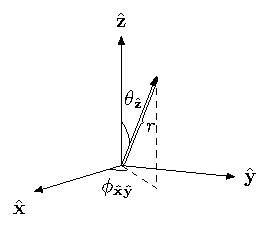
\includegraphics[width = 1.0\textwidth]{../figures/frames/frames_a.pdf}
   \caption{$\hat{\mathbf{z}}\mb{\hat{x}}$ spherical coordinates.}
   \label{fig:frames_a}
 \end{subfigure}%
 ~
 \begin{subfigure}[t]{0.25\textwidth}
   \centering
   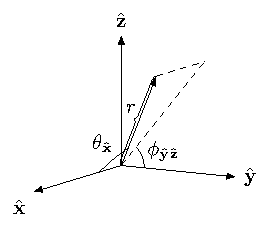
\includegraphics[width = 1.0\textwidth]{../figures/frames/frames_b.pdf}
   \caption{$\hat{\mathbf{x}}\mb{\hat{y}}$ spherical coordinates.}
   \label{fig:frames_b}
 \end{subfigure}%
~
 \begin{subfigure}[t]{0.25\textwidth}
   \centering
   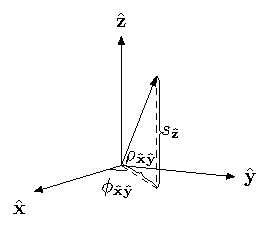
\includegraphics[width = 1.0\textwidth]{../figures/frames/frames_d.pdf}
   \caption{$\hat{\mathbf{z}}\mb{\hat{x}}$ cylindrical coordinates.}
   \label{fig:frames_c}
 \end{subfigure}%
  \begin{subfigure}[t]{0.25\textwidth}
   \centering
   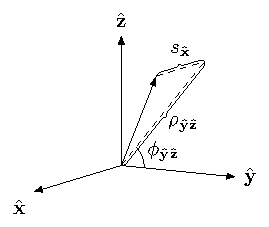
\includegraphics[width = 1.0\textwidth]{../figures/frames/frames_c.pdf}
   \caption{$\hat{\mathbf{x}}\mb{\hat{y}}$ cylindrical coordinates.}
   \label{fig:frames_c}
 \end{subfigure}%

 \caption{Coordinate systems.}
 \label{fig:frames}
\end{figure*}

\subsubsection{Electric Field In The Back Focal Plane}
We can model the action of the objective on the electric fields by a position
dependent rotation matrix.

A right handed rotation about a vector $\mh{u} = u_x\mh{x} + u_y\mh{y} + u_z\mh{z}$
by angle $\theta$ can be represented by the rotation matrix
\begin{align}
\tilde{\mb{R}}_{\mh{u}}(\theta) &= \begin{bmatrix}
  \cos\theta + u_x^2(1 - \cos\theta) & u_xu_y(1 - \cos\theta) - u_z\sin\theta & u_xu_z(1 - \cos\theta) + u_y\sin\theta\\
  u_yu_x(1-\cos\theta) + u_z\sin\theta & \cos\theta + u_y^2(1 - \cos\theta) & u_yu_z(1 - \cos\theta) - u_x\sin\theta\\
  u_zu_x(1 - \cos\theta) - u_y\sin\theta & u_zu_y(1 - \cos\theta) + u_x\sin\theta &  \cos\theta + u_z^2(1 - \cos\theta)
\end{bmatrix}\\
\tilde{\mb{R}}_{\mh{u}}(\theta) &= \cos\theta\tilde{\mb{I}} + \sin\theta\left[\mh{u}\right]_{\times} + (1 - \cos\theta)\mh{u}\mh{u}^{\dagger}
\end{align}
where $\left[\mh{u}\right]_{\times}$ is the cross product matrix of $\mh{u}$ \cite{rotation}.

A lens rotates electric fields into the plane perpendicular to the optic
axis (equivalently, a lens rotates each ray parallel to the optic axis). The
rotation matrix that describes the rotation of the electric field at $\mh{r}$ by a
lens with optic axis $\mh{s}$ is
\begin{align}
  \tilde{\mb{R}}_{\mh{r}\times\mh{s}}(\text{acos}(\mh{r}\cdot\mh{s})) = (\mh{r}\cdot\mh{s})\tilde{\mb{I}} + \sqrt{1 - (\mh{r}\cdot\mh{s})^2}\left[\mh{r}\times\mh{s}\right]_{\times} + (1 - \mh{r}\cdot\mh{s})(\mh{r}\times\mh{s})(\mh{r}\times\mh{s})^{\dagger}
\end{align}

To conserve energy, we need to multiply the rotation matrix by a factor of $\sqrt{\frac{n_1}{n_0(\mh{r}\cdot\mh{s})}}$ \cite{nov} where $n_0$ is the index of refraction of the lens. Finally, we truncate the electric fields to simulate the finite numerical aperture of the lens. The final matrix that represents the lens is given by
\begin{align}
  \mb{\tilde{O}}_{\mh{s}} = \sqrt{\frac{n_1}{n_o(\mh{r}\cdot\mh{s})}}\Pi\left(\frac{|\mb{r} - (\mb{r}\cdot\mh{s})\mh{s}|}{\rho_{\text{max}}}\right)  \tilde{\mb{R}}_{\mh{r}\times\mh{s}}(\text{acos}(\mh{r}\cdot\mh{s}))\label{eq:2}
\end{align}
  where $|\mb{r} - (\mb{r}\cdot\mh{s})\mh{s}|$ is the shortest distance from $r$ to the optic axis, $\rho_{\text{max}}$ is the
  radius of the objective lens
  ($\rho_{\text{max}} =
  f_{\text{obj}}\tan\left(\arcsin\left(\frac{\text{NA}}{n_1}\right)\right)$),
  and
\begin{align}
  \Pi(x) = \begin{cases} 1, |x| < 1\\ 0, |x| > 1\end{cases}.
\end{align}


Now that we can compute the effect of the objective lens, we can compute the
electric field in the back focal plane
\begin{align}
  \mb{E}_{\text{bfp}} &= \mb{\tilde{O}}_{\text{obj}}\tensor{\mathbf{G}}_{FF}\bs{\mu}
  \end{align}
  If we place a polarizing element in the back focal plane, $\mb{E}_{\text{bfp}}$ will
  be projected onto the pass direction of the polarizing element. 

  
The intensity in the back focal plane is given by
\begin{align}
  I_{\text{bfp}}(\mb{r}) = \mb{E}_{\text{bfp}}^{\dag}\mb{E}_{\text{bfp}}
  = |\mb{E}_{\text{bfp}}|^2.
\end{align}

\subsubsection{Electric Field In The Image Plane}
If $f_{\text{obj}} \ll f_{\text{tube}}$, then the paraxial approximation applies
and
\begin{align}
  \mb{E}_{\text{img}}(\mb{r''}) = \mathcal{F}_{3D}\{\mb{E}_{\text{bfp}}\}|_{\lambda f_{\text{tube}}} = \int_{\mathbb{R}^3}\mb{E}_{\text{bfp}}e^{-i\frac{k}{f_{\text{tube}}}\mb{r}\cdot\mb{r''}}d\mb{r}.
\end{align}
where $\mb{r''}$ is the position in the image plane. If we place a polarizing
element in the imaging plane, $\mb{E}_{\text{img}}$ will be projected onto
the pass direction of the polarizing element.

Finally, the intensity in the image plane is
\begin{align}
  I_{\text{img}}(\mb{r''}) = \mb{E}_{\text{img}}^{\dag}\mb{E}_{\text{img}}
  = |\mb{E}_{\text{img}}|^2.
\end{align}

Notice that we take the 3D Fourier transform instead of the usual 2D. The
objective lens rotates the electric fields to the transverse plane, so the
usual 2D FT is equivalent to the 3D FT evaluated in any transverse plane. I've
used the 3D FT to simplify the notation and show that we can use the same
operation for any optic axis.

Also note that the Fourier transform is acting on a vector field instead of the
usual scalar field. The FT of a vector field is just the usual scalar FT applied
to each component of the vector.

\subsection{Current Techniques}
\subsubsection{Single View}
If the optic axis is along the $\mh{z}$ axis and we have an infinite numerical aperture, the objective lens matrix reduces to
\begin{align}
  \mb{\tilde{O}}_{\mb{\hat{z}},\text{obj}} &= 
  \sqrt{\frac{n_1}{n_o\cos(\theta_z)}}\begin{bmatrix}
    \cos(\theta_z)\cos^2(\phi_{xy}) + \sin^2(\phi_{xy}) & (\cos(\theta_z) - 1)\sin(\phi_{xy})\cos(\phi_{xy}) & -\sin(\theta_z)\cos(\phi_{xy})\\
    (\cos(\theta_z) - 1)\sin(\phi_{xy})\cos(\phi_{xy}) & \cos(\theta_z)\sin^2(\phi_{xy}) + \cos^2(\phi_{xy}) & \sin(\theta_z)\sin(\phi_{xy})\\
    \sin(\theta_z)\cos(\phi_{xy}) & \sin(\theta_z)\sin(\phi_{xy}) & \cos(\theta_z)
  \end{bmatrix}. \label{eq:1}
\end{align}
Equation \ref{eq:1} is identical to equation 11 in \cite{backer} and equation 2
in Fourkas' paper \cite{fourkas}. Fourkas sums the intensity over the entire
image plane, while we consider the complete imaging model. In our formulation,
we combine the effects of NA, the apodization, and the rotation of the lens into
a single matrix $\tilde{\mb{O}}$ (Equation \ref{eq:2}).

\subsubsection{Back Focal Plane Manipulation}
The Moerner group has used a variety of phase and amplitude masks in the back
focal plane of the detection path \cite{backer}. These techniques effectively change
the point spread function of the detection system. 

\subsection{Possible Techniques}
\subsubsection{Arbitrary Views Of A Dipole Near The Focal Point}
The work in the general analysis section allows us to calculate the images created by
multiple views along arbitrary optic axes. This allows us to analyze new geometries
like diSPIM. 

\section{Complete Forward Model}
Combining all of the previous sections gives the complete forward
model:
\begin{align}
  I_{\text{img}}(\mb{r''}) = \left|\mathcal{F}_{3D}\left\{
    \mb{\tilde{O}}_{\text{obj}}\tensor{\mathbf{G}}_{FF}\tensor{\bs{\alpha}}\mb{E}_{\text{in}}
  \right\}
  \right|^2.\label{eq:5}
\end{align}
where
\begin{align*}
  \mb{E}_{\text{in}}\ & \text{is the incident electric field pattern established by the illumination optics. It is a function of the input light}\\ & \text{source, input light pattern (phase, amplitude, polarization modulation), and input light optics (spherical,}\\ & \text{cylindrical lens). }\\
  \tensor{\bs{\alpha}}\ & \text{is the polarizability tensor. It is a function of
                          the fluorophore type and the fluorophore's orientation.}\\
  \tensor{\mb{G}}_{FF}\ & \text{is the Green's tensor that generates the electric fields
                          far from the induced dipole moment. It is a function}\\ & \text{of the
                          dipole moment's position and the refractive index of the
                          medium.}\\
  \mb{\tilde{O}}_{\text{obj}}\ & \text{is the matrix that describes the action of the
                                 objective lens. It is a function of the objective's
                                 focal length,}\\ &\text{NA, and optic axis.}
\end{align*}


\bibliography{report}{}
\bibliographystyle{unsrt}

\end{document}

